%%%%%%%%%%%%%%%%%%%%%%%%%%%%%%%%%%%%%%%%%%%%%%%%%%%%%%%%%%%%%%%%%%%%%%%%%%%
%
% Plantilla para un art�culo en LaTeX en espa�ol.
%
%%%%%%%%%%%%%%%%%%%%%%%%%%%%%%%%%%%%%%%%%%%%%%%%%%%%%%%%%%%%%%%%%%%%%%%%%%%

\documentclass{article}

% Esto es para poder escribir acentos directamente:
\usepackage[latin1]{inputenc}
% Esto es para que el LaTeX sepa que el texto est� en espa�ol:
\usepackage[spanish]{babel}

% Paquetes de la AMS:
\usepackage{amsmath, amsthm, amsfonts}

% Paquete para generar grafos
\usepackage{tikz}
% Paquete para tratar con im�genes
\usepackage{graphicx}

% Teoremas
%--------------------------------------------------------------------------
\newtheorem{thm}{Teorema}[section]
\newtheorem{cor}[thm]{Corolario}
\newtheorem{lem}[thm]{Lema}
\newtheorem{prop}[thm]{Proposici�n}
\theoremstyle{definition}
\newtheorem{defn}[thm]{Definici�n}
\theoremstyle{remark}
\newtheorem{rem}[thm]{Observaci�n}

% Atajos.
% Se pueden definir comandos nuevos para acortar cosas que se usan
% frecuentemente. Como ejemplo, aqu� se definen la R y la Z dobles que
% suelen representar a los conjuntos de n�meros reales y enteros.
%--------------------------------------------------------------------------

\def\RR{\mathbb{R}}
\def\ZZ{\mathbb{Z}}

% De la misma forma se pueden definir comandos con argumentos. Por
% ejemplo, aqu� definimos un comando para escribir el valor absoluto
% de algo m�s f�cilmente.
%--------------------------------------------------------------------------
\newcommand{\abs}[1]{\left\vert#1\right\vert}

% Operadores.
% Los operadores nuevos deben definirse como tales para que aparezcan
% correctamente. Como ejemplo definimos en jacobiano:
%--------------------------------------------------------------------------
\DeclareMathOperator{\Jac}{Jac}

%--------------------------------------------------------------------------
\title{Memoria de la pr�ctica 5 de RPI1}
\author{Jose Fabrizio Alcaraz Escobar y Daniel Mihai Rece}

\begin{document}
\maketitle


\section{Introducci�n}

Comenzamos la pr�ctica haci�ndonos con las herramientas necesarias: \b{hcitool} para gestionar la interfaz Bluethoot y \b{gatttool} para la conexi�n e iteracci�n con la tabla GATT. En este caso, nuestro dispositivo constar� del nombre configurado "ESP\_GATS\_FADA" y la MAC por defecto c4:dd:57:5b:fd:12 (tal y como se muestra en la imagen \ref{lescan}).

\begin{figure}[!h]%
  \centering
  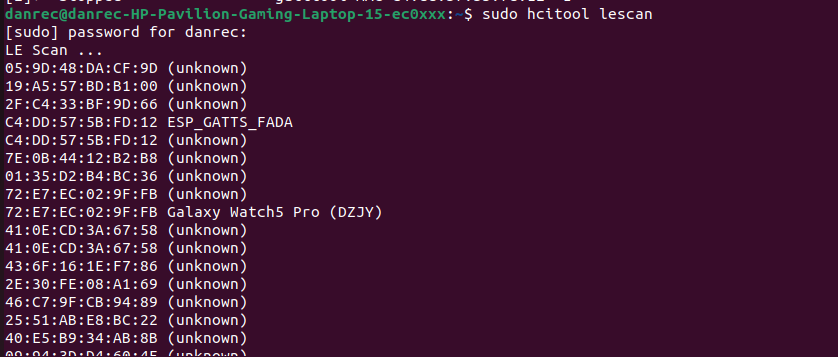
\includegraphics[width=60mm]{hcitool-lescan.png}
  \caption{CLI hcitool lescan}
  \label{lescan}
\end{figure}

Una vez accedemos al dispositivo haciendo uso de gatttool, procedemos a conectarnos mediante el comando connect para inmediatamente lanzar help y estudiar los comandos disponibles. Nuestro objetivo es identificar la caracter�stica asociada a la constante GATTS\_CHAR\_UUID\_TEST\_A de valor $0xFF01$ de nuestro programa, que, a su vez, es la que gestiona las variables char\_value que vamos a querer leer. Una vez identificada gracias a los valores precedentes al primer gui�n de la uuid (consultar imagen \ref{char}), procedemos a leer el valor de la variable anteriormente mencionada por medio del comando char-read-hnd seguido del "char value handle" de la caracter�stica.

\begin{figure}[!h]%
  \centering
  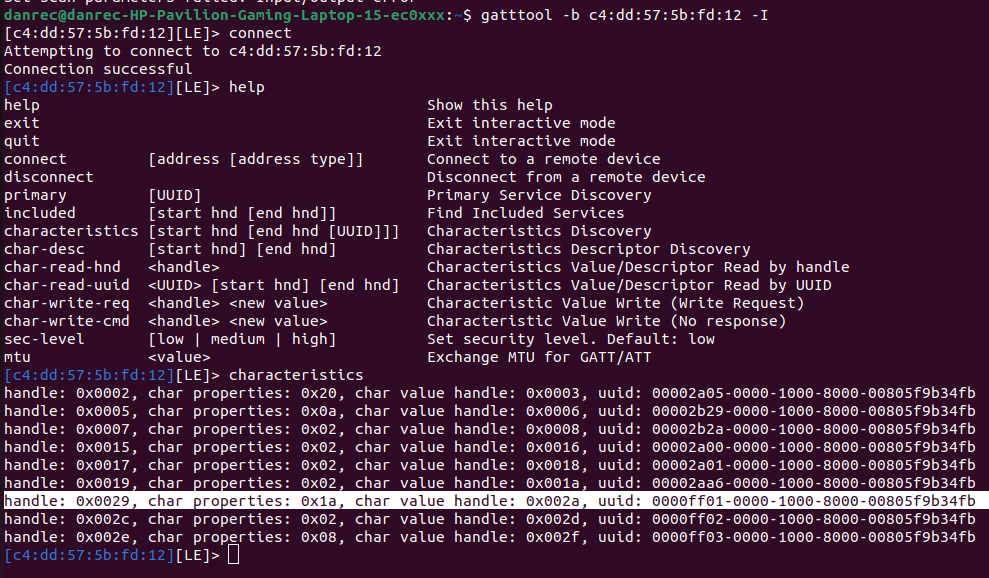
\includegraphics[width=60mm]{char-identifi.png}
  \caption{CLI gatttool char identification}
  \label{char}
\end{figure}

Tras haber accedido a estos valores, observamos que tenemos 2 maneras de modificarlos. Una de ellas es por medio del programa base o main, al que accederemos y modificaremos su c�digo para volver a compilar y flashear nuestra tarjeta ESP-32. La segunda opci�n (no es permanente y volver� al valor original tras la desconexi�n de la placa) consiste en usar la propia consola que nos ofrece gatttool: haciendo uso del comando char-write-cmd seguido del "char value handle" de la caracter�stica y proporcion�ndole un nuevo valor.


Para finalizar los preparativos, accedemos al siguiente "char value handle", asociado a la configuraci�n de la caracter�stica anterior. Esto nos permite enviar comandos de configuraci�n que permitan realizar x o y acci�n, se mostrar� en el ejercicio con m�s detalle.



\section{Ejercicio}

El ejercicio consiste en programar una tarea que monitorice par�metros (en este caso aleatorios) y los muestre a todo aquel interesado en obtenerlo por medio de la herramienta gatttool. Para este fin, creamos una tarea que cada segundo ir� actualizando la variable char-value y la enviar� a aquel que se suscriba. Para realizar una suscripci�n, el cliente tendr� que escribir un comando de configuraci�n 0100; para cancelar la suscripci�n, bastar� con enviar un comando de configuraci�n 0000. En las im�genes \ref{rw} y \ref{t} adjuntas, se muestra como funcionan ambos comandos desde la perspectiva del cliente y del servidor respectivamente.

\begin{figure}[!h]%
  \centering
  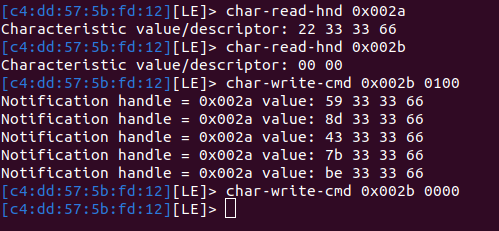
\includegraphics[width=60mm]{read-write-sub-unsub.png}
  \caption{Client (sub-unsub)scribe}
  \label{rw}
\end{figure}
\begin{figure}[!h]%
  \centering
  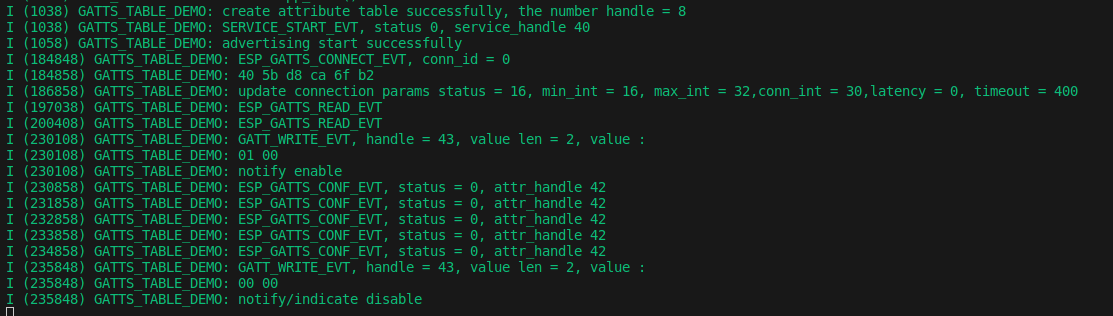
\includegraphics[width=60mm]{teminal.png}
  \caption{Server (sub-unsub)scribe}
  \label{t}
\end{figure}





\end{document}
